% !TEX root = ../YourName-Dissertation.tex

\chapter{Neutrinos and Neutrino Masses}

\section{Introduction}

\section{Neutrinos}

\section{Neutrino Oscillations}

\begin{figure}[htbp]
    \centering
    \includegraphics[width=0.6\textwidth]{figs/Chapter-2/230227_chap2_nu_hierarchy.png}
    \caption{Caption}
    \label{fig:nu_hierarchy}
\end{figure}

\section{Neutrino Mass}

\subsection{Limits from Cosmology}

\begin{figure}[htbp]
    \centering
    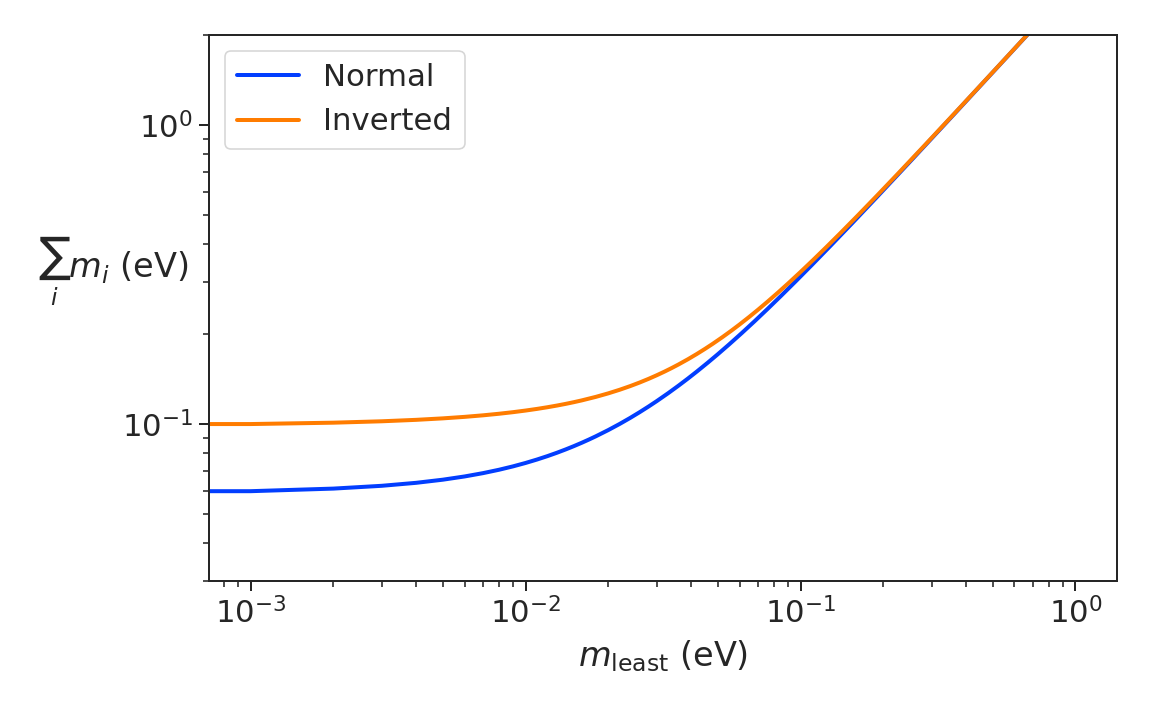
\includegraphics[width=0.7\textwidth]{figs/Chapter-2/230301_cosmology_nu_mass_observable.png}
    \caption{Caption}
    \label{fig:nu_mass_cosmo}
\end{figure}


%\begin{figure}[htbp]
%    \centering
%    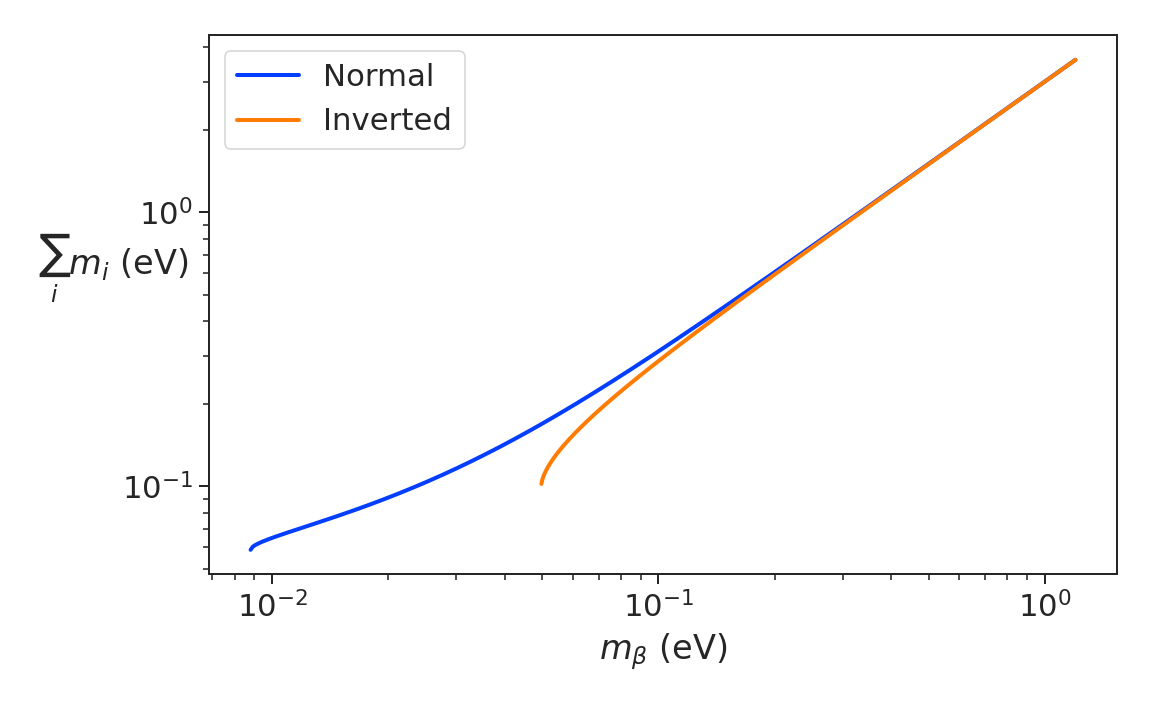
\includegraphics[width=0.7\textwidth]{figs/Chapter-2/230301_sum_nu_mass_vs_m_beta.png}
%    \caption{Caption}
%    \label{fig:nu_mass_cosmo_vs_nu_beta}
%\end{figure}
%\lipsum[1]

\subsection{Limits from Neutrinoless Double Beta-decay Searches}

\begin{figure}[htbp]
    \centering
    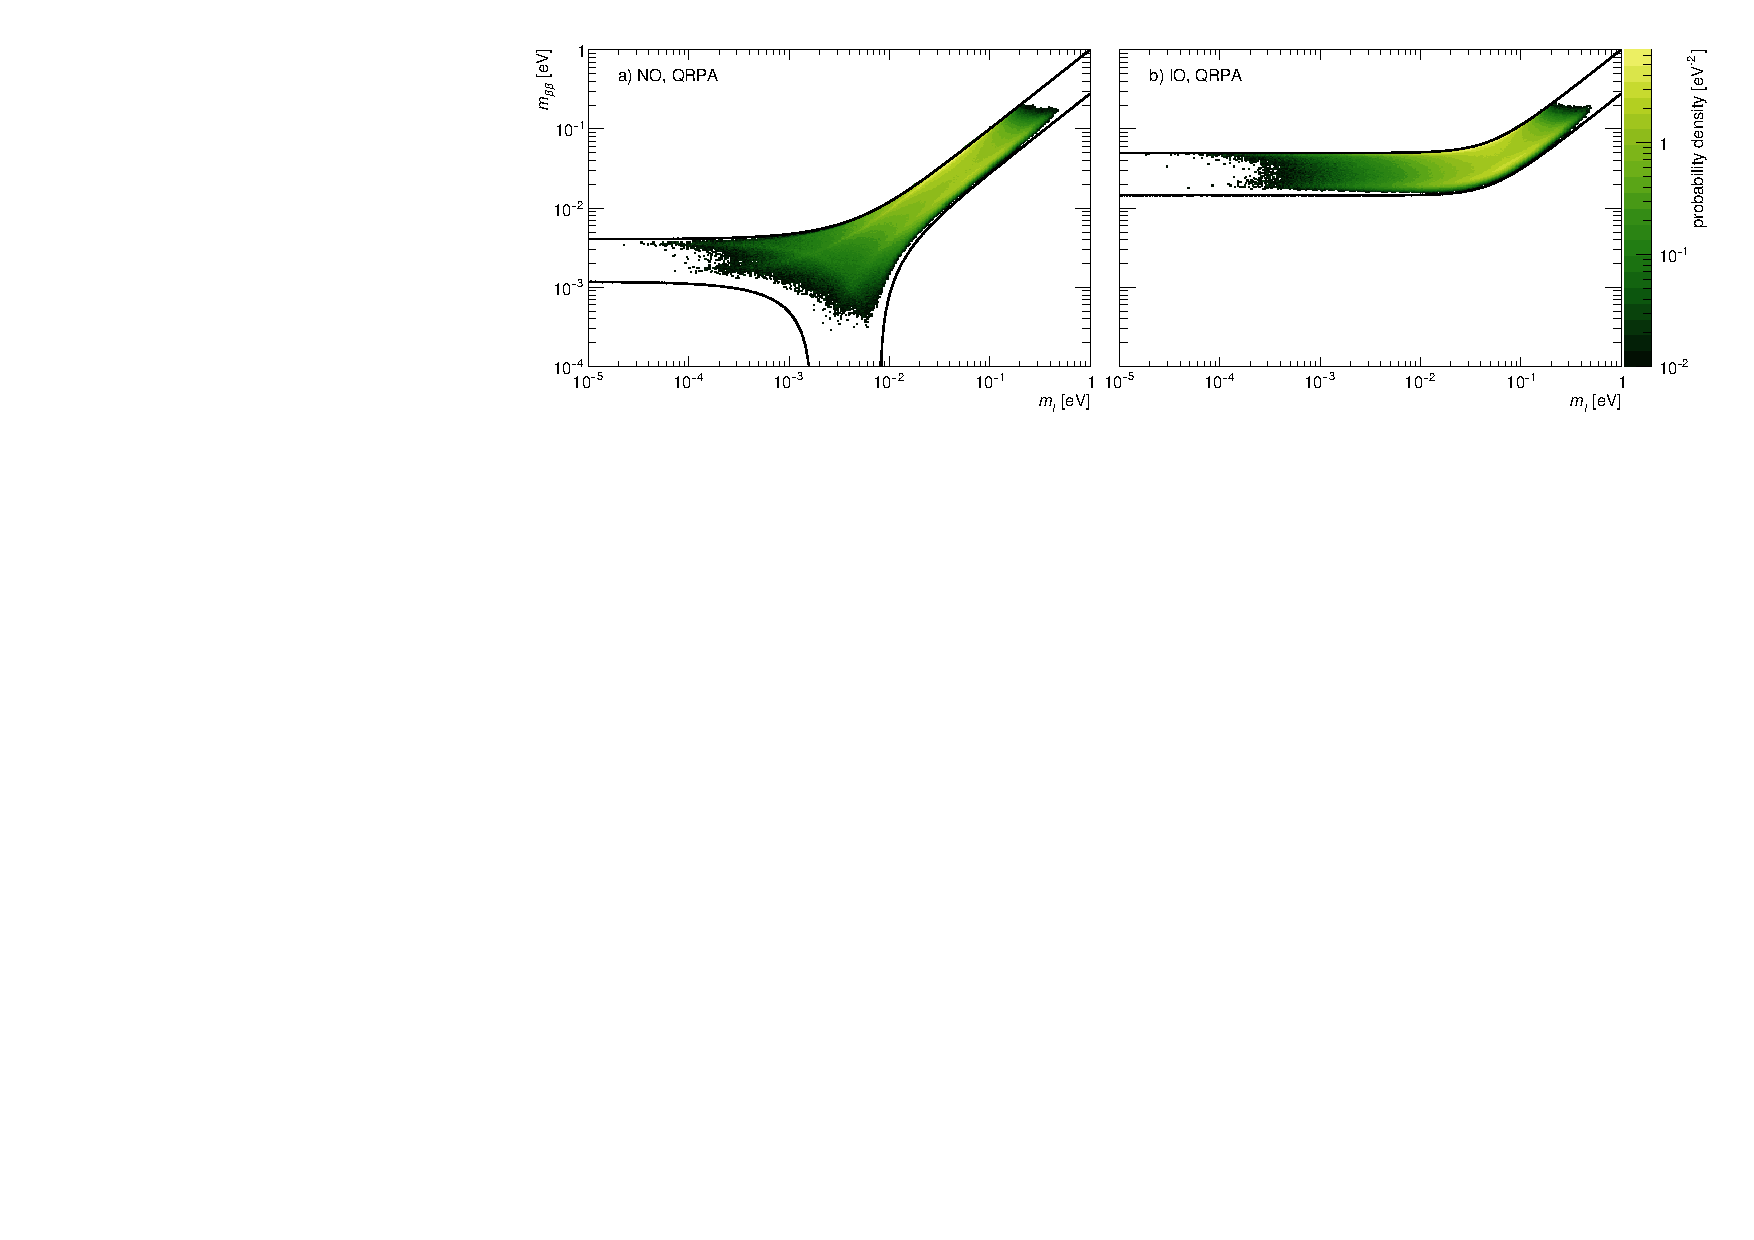
\includegraphics[width=1.0\textwidth]{figs/Chapter-2/230228_nu_mass_0nbb.pdf}
    \caption{Caption}
    \label{fig:nu_mass_0nbb_posterior}
\end{figure}

\begin{figure}[htbp]
    \centering
    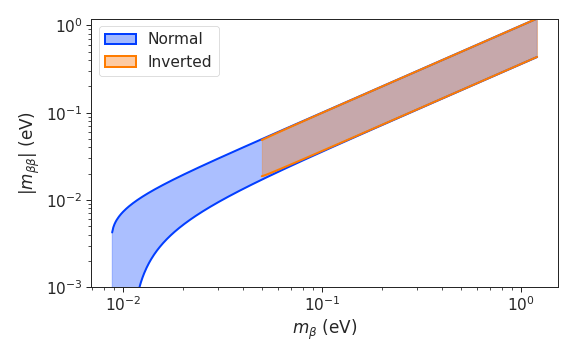
\includegraphics[width=0.7\textwidth]{figs/Chapter-2/230301_mbb_vs_mb.png}
    \caption{Caption}
    \label{fig:nu_mass_0nbb_vs_nu_beta}
\end{figure}

\subsection{Kinematic Measurements of the Neutrino Mass}

\begin{figure}[htbp]
    \centering
    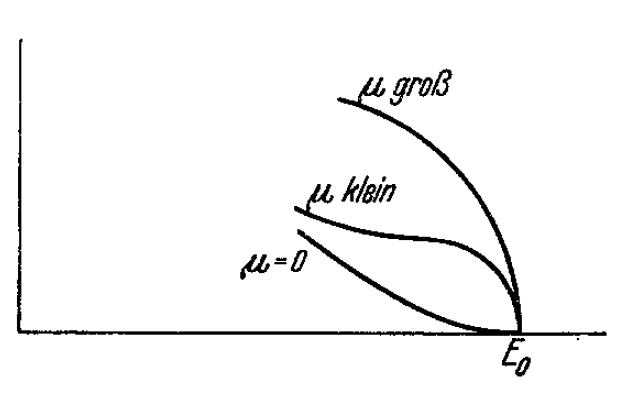
\includegraphics[width=0.7\textwidth]{figs/Chapter-2/Fermi.png}
    \caption{Caption}
    \label{fig:fermi_original_b_spectrum}
\end{figure}

\begin{figure}[htbp]
    \centering
    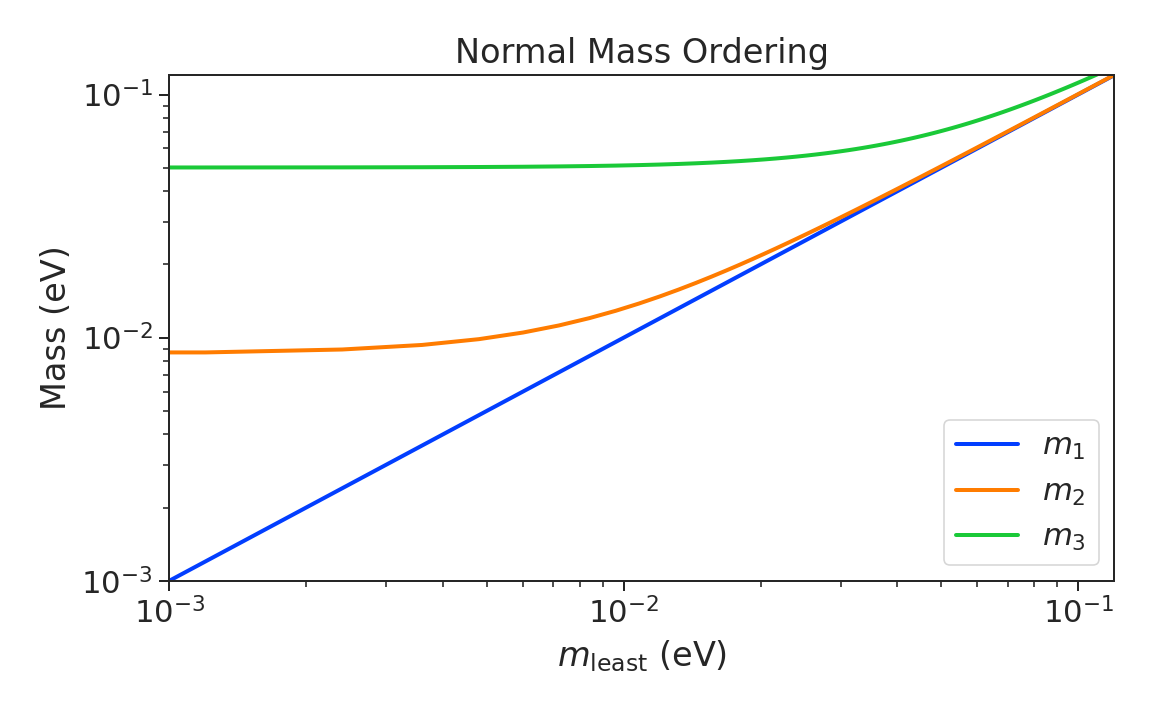
\includegraphics[width=0.7\textwidth]{figs/Chapter-2/230302_mass_estate_vals_normal.png}
    \caption{Caption}
    \label{fig:mass_estates_normal}
\end{figure}

\begin{figure}[htbp]
    \centering
    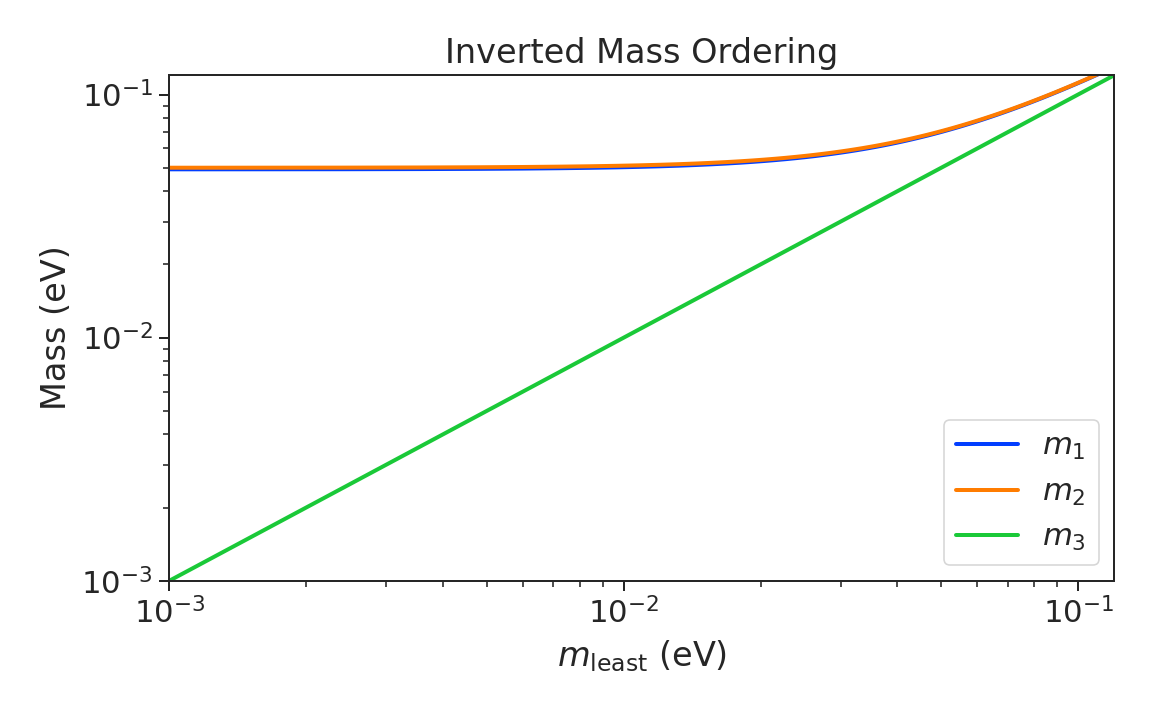
\includegraphics[width=0.7\textwidth]{figs/Chapter-2/230302_mass_estate_vals_inverted.png}
    \caption{Caption}
    \label{fig:mass_estates_inverted}
\end{figure}

\section{Neutrino Mass Measurements Using Tritium Beta-decay Spectroscopy}

\begin{figure}[htbp]
    \centering
    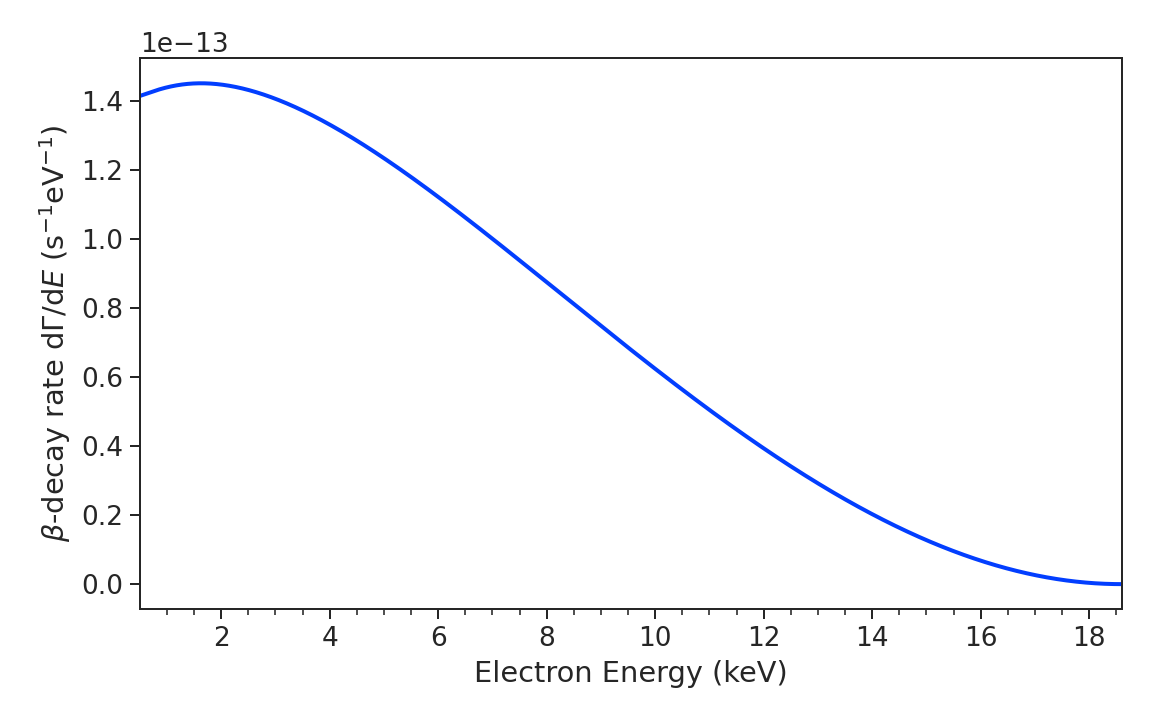
\includegraphics[width=0.7\textwidth]{figs/Chapter-2/230302_atomic_tritium_spectrum.png}
    \caption{Caption}
    \label{fig:atomic_tritium_spectrum}
\end{figure}

\begin{figure}[htbp]
    \centering
    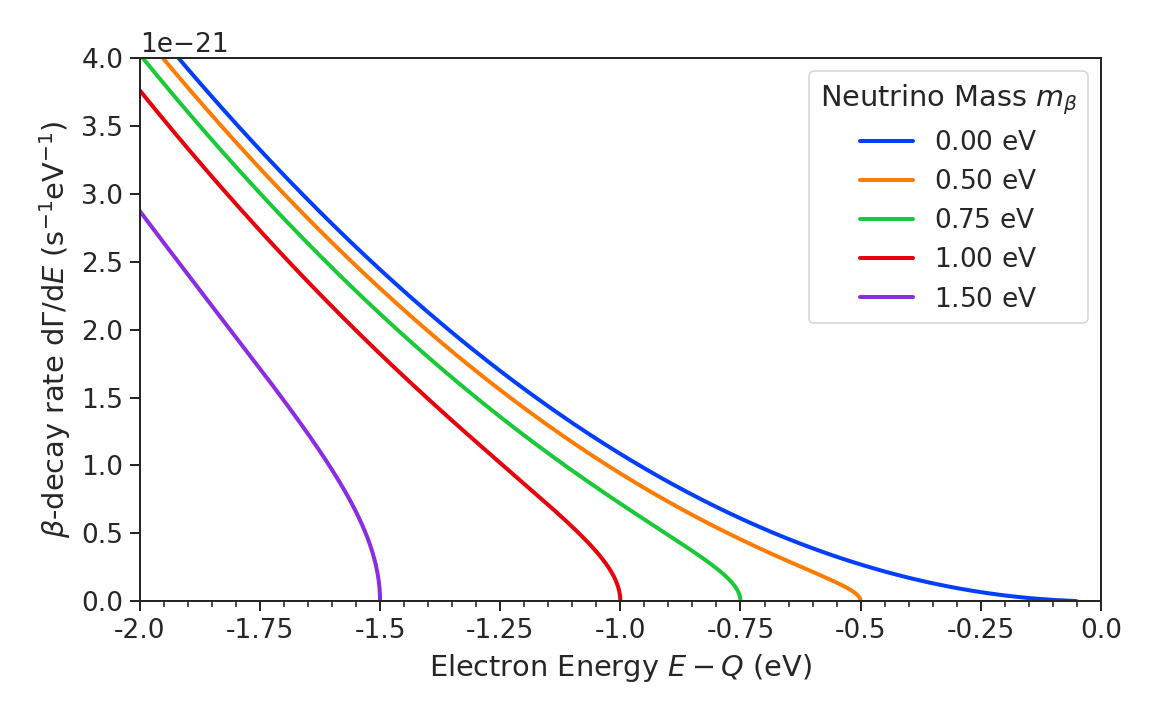
\includegraphics[width=0.7\textwidth]{figs/Chapter-2/230302_atomic_tritium_spectrum_near_endpoint.png}
    \caption{Caption}
    \label{fig:atomic_tritium_endpoint}
\end{figure}
